\documentclass[xcolor=dvipsnames]{beamer} 


\usetheme[
          showdate=true,                     % show the date on the title page
          alternativetitlepage=true,         % Use the fancy title page.
          titlepagelogo=general_figures/shell,              % Logo for the fir\
st page.
          ]{UMD}

%\usetheme{Rochester}

%\usepackage{beamerthemesplit}
\usepackage{xmpmulti}

\usepackage{graphicx,float,wrapfig, bbm}
\usepackage{amsfonts, bbold, comment}
\usepackage{mdwlist}
\usepackage{subfigure}
\usepackage{colortbl}

\usepackage{multirow}


\newcommand{\fsi}[2]{
\begin{frame}[plain]
\vspace*{-1pt}
\makebox[\linewidth]{\includegraphics[width=\paperwidth]{#1}}
\begin{center}
#2
\end{center}
\end{frame}
}


\newcommand{\e}[2]{\mathbb{E}_{#1}\left[ #2 \right] }
\newcommand{\ind}[1]{\mathbb{I}\left[ #1 \right] }
\newcommand{\ex}[1]{\mbox{exp}\left\{ #1\right\} }
\newcommand{\g}{\, | \,}
\newcommand{\citename}[1]{#1 }

\newcommand{\gfxs}[2]{
\begin{center}
	\includegraphics[width=#2\linewidth]{simtrans/#1}
\end{center}
}

\newcommand{\gfxq}[2]{
\begin{center}
	\includegraphics[width=#2\linewidth]{qb/#1}
\end{center}
}



%\usecolortheme{ucdblack}
\title[HCQA]{Human-Computer Question Answering: \\ 
NIPS 2017 Competition}
\author{ Jordan Boyd-Graber et al.}
\date{2017}

\institute[Maryland] % (optional, but mostly needed)
{University of Maryland}

\begin{document}

\frame{
\titlepage
\tiny
}


\begin{frame}{Human-Computer Question Answering}

  \begin{itemize}
    \item Pit machine learning algorithms against humans
    \item Fun task for human participants
    \item Good system for discriminating depth and confidence of
      algorithms
    \item Knowledge and language comprehension needed to do well
    \item Simple approaches work well if you have the whole question
  \end{itemize}

\end{frame}


\begin{frame}
	\frametitle{How is this different from Jeopardy?}

	\begin{columns}
		\column{.5\linewidth}

		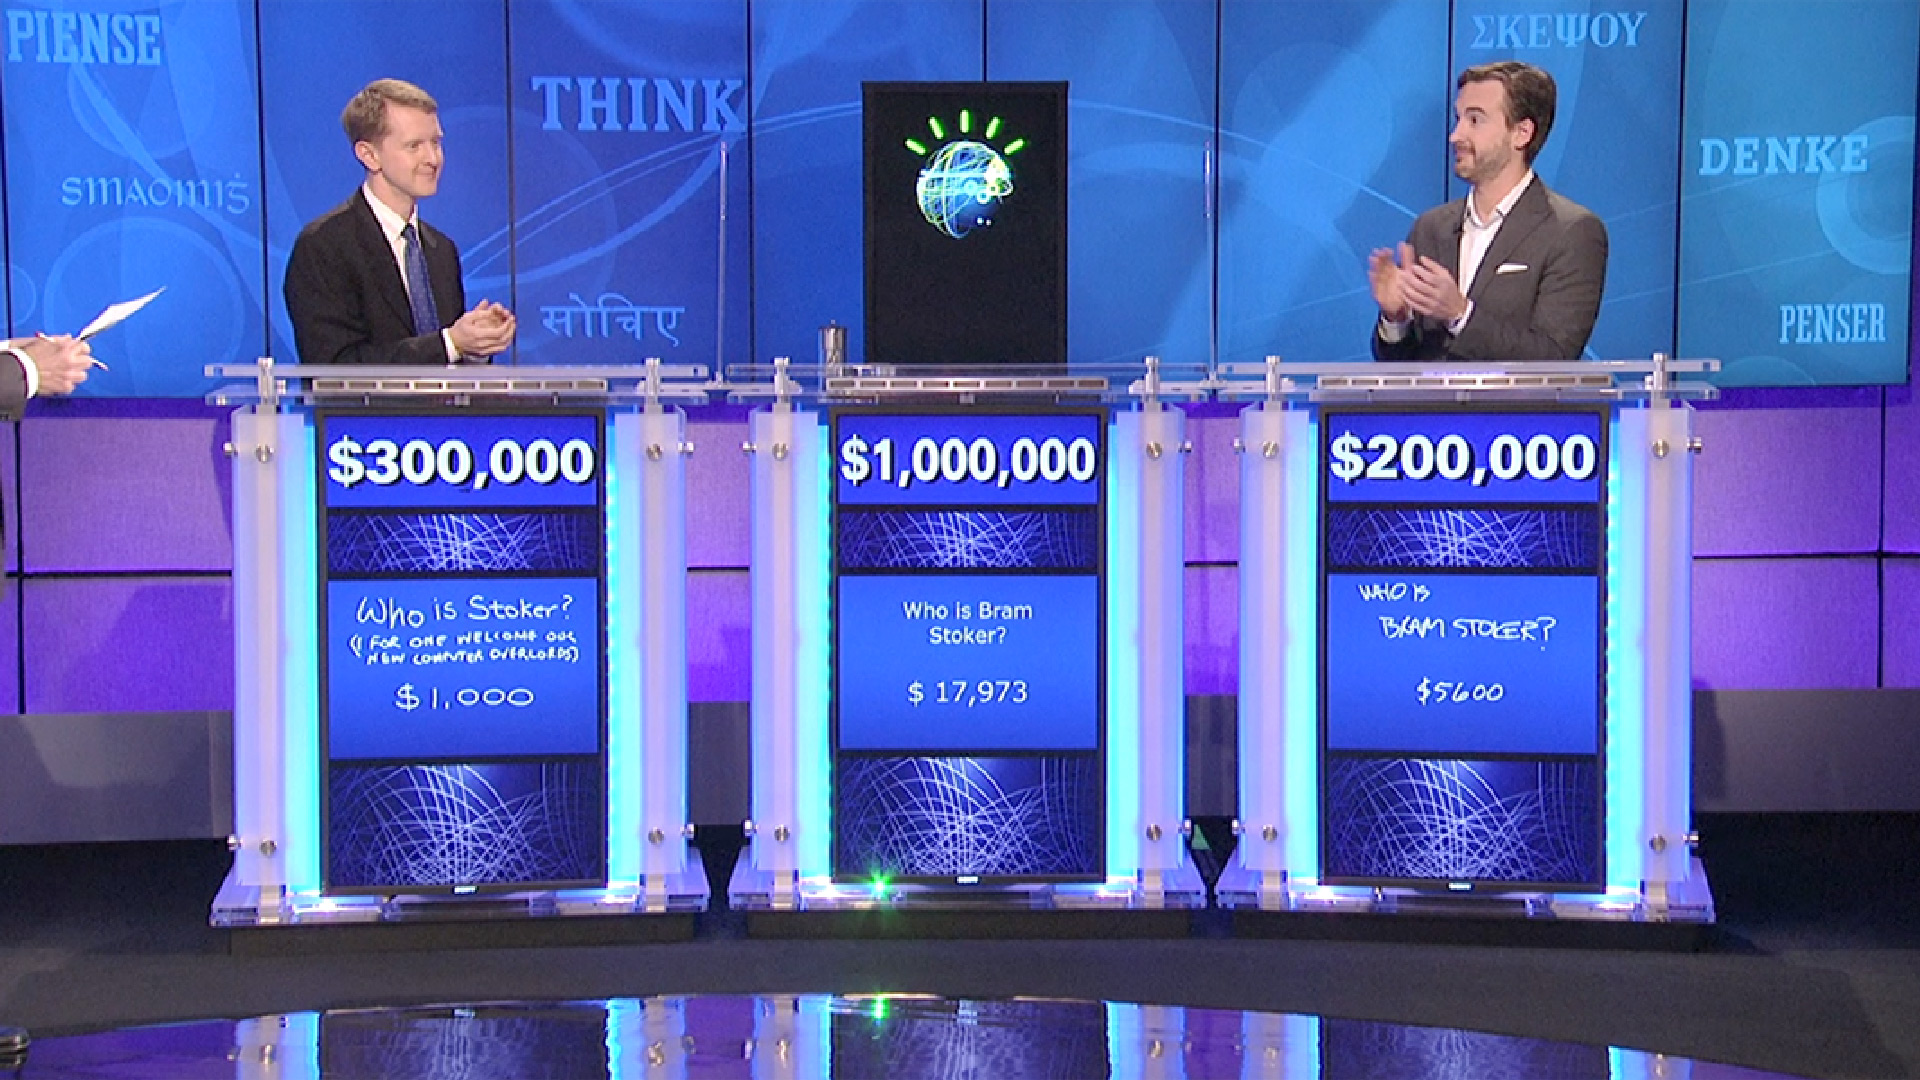
\includegraphics[width=1.0\linewidth]{qb/jeopardy}


		\column{.5\linewidth}
		\begin{itemize}
			\item This is {\bf not} Jeopardy
			\item There are buzzers, but players only buzz
                          at the question end
			\item Doesn't discriminate knowledge
			\item Quiz bowl is pyramidal
                        \item Watson must decide to answer {\bf once}, after
                          complete question
                        \item Quiz Bowl: decide after each word
		\end{itemize}

	\end{columns}

\end{frame}



\begin{frame}{Matching Entites Across Sentences}

\begin{block}{\only<2->{Magic Flute}}

    At its premiere, \alert<3>{the librettist of this opera} portrayed
    \alert<4>{a character who asks for a glass of wine with his dying wish}. \alert<4>{That
    character} in this opera is instructed to ring some bells to summon
    his love. At its beginning, \alert<5>{a man} who claims to have killed a (*)
    serpent has a padlock put on \alert<5>{his} mouth because of \alert<5>{his} lying. The
    plot of this opera concerns a series of tests that \alert<5>{Tamino} must
    undergo to rescue Tamina from Sorastro. For 10 points, name this
    Wolfgang Mozart opera titled for \alert<6>{an enchanted woodwind instrument}.
\end{block}



\only<3-4>{{\bf Not all references are named (\alert<3>{Emanuel
      Schikaneder}, \alert<4>{Papageno})}}
\only<5>{Need to be able to match pronouns across sentences (or have
  deep world knowledge)}
\only<6>{Requires semantic knowledge}
\end{frame}




\begin{frame}{How the shared task works}

\begin{columns}
  \column{.3\linewidth}
  \gfxq{bamber}{.8}

  \column{.65\linewidth}
  \begin{itemize}
    \item<3-> Hi! Available questions are \texttt{[1,2,3,4]}
    \item<5-> It's \texttt{Extremism}
    \item<7-> It's \texttt{in}
    \item<9-> It's \texttt{the}
    \item<11-> Got it!  You've answered Question 1 at Position
      3 with \texttt{Barry\_Goldwater}
  \end{itemize}

\end{columns}


\begin{columns}

  \column{.65\linewidth}
  \begin{itemize}
    \item<2-> I'm User~1.  I’d like to play!
    \item<4-> I’d like to hear Word~1 of Question 1
    \item<6-> I’d like to hear Word~2 of Question 1
    \item<8-> I’d like to hear Word~3 of Question 1
    \item<10-> I’d like to answer Question 1 with
      \texttt{Barry\_Goldwater}
    \end{itemize}
  \column{.3\linewidth}
  \only<2->{\gfxq{buzzer}{.5}}
\end{columns}

\end{frame}


\begin{frame}{It's Easy to Get Started}

  \begin{itemize}
    \item Perform relatively well at the task
    \item Easy to improve
    \item Designed for students taking graduate machine learning
  \end{itemize}

\end{frame}

\begin{frame}{Timeline}

  \begin{itemize}
    \item August 1, 2017: Reference systems and data available
    \item September 1, 2017: Server available with development data
    \item October 8, 2017: Competition data available
    \item October 15, 2017: Deadline for submitting machine entries
    \item October 20, 2017: Preliminary results released to teams 
    \item November 1, 2017: Deadline for submitting white papers
    \item Early December: Live competition at NIPS 
  \end{itemize}

\end{frame}


\begin{frame}{History of Competition}

		\begin{columns}
			\column{.25\linewidth}
				\gfxq{colby_jeo}{1.0}
                                Colby Burnett:
                                \$375,000
			\column{.25\linewidth}
				\gfxq{ben_jeo}{1.0}
                                Ben Ingram:
                                \$427,534
			\column{.25\linewidth}
				\gfxq{alex_jeo}{1.0}
                                Alex Jacobs: \$151,802
			\column{.25\linewidth}
				\gfxq{kristin_jeo}{1.0}
                                Kristin Sausville: \$95,201
		\end{columns}

                \pause

                \begin{center}
                End result: 200-200 tie!
                \end{center}

\end{frame}

\fsi{qb/hsnct1}{}
\fsi{qb/jennings}{23. October 2015, Seattle}
\fsi{qb/jennings_handshake}{QANTA 300--160}
\fsi{qb/nasat}{Humans 345--145}
\fsi{qb/hsnct_2016}{Humans 190--155}
\fsi{qb/atlanta}{QANTA 260--215}



\begin{frame}{Find out More!}

		\begin{itemize}
			\item Code: \url{http://github.com/Pinafore/qb}
                        \item Shared Task \url{hcqa.boydgraber.org}
		\end{itemize}

\end{frame}


\begin{frame}{Who we are}


	\begin{columns}
		\column{.4\linewidth}
                \begin{itemize}
                  \item \alert<1>{Jordan Boyd-Graber}
                  \item \alert<2>{Mohit Iyyer}
                  \item \alert<3>{Pedro Rodriguez}
                  \item \alert<4>{He He}
                   \item \alert<5>{Hal Daum\'e III}
                \end{itemize}


		\column{.6\linewidth}

                \only<1>{
			\begin{block}{Jordan Boyd-Graber}

			\begin{itemize}
				\item Assoc. Professor, UMD
				\item Former quiz bowl player at
                                  Caltech and
                                  Princeton 
                                \item \url{boydgraber.org}        
                                \item @boydgraber                        
			\end{itemize}
			\gfxq{jordan_qb}{.5}
			\end{block}
			}


\only<2>{
			\begin{block}{Mohit Iyyer}
			\begin{itemize}
                                \item Postdoc, AI$^2$
                                \item 2018: Assistant Professor
                                  at U Mass Amherst
				\item National Champion, 2008 HSNCT
                                \item
                                  \url{https://cs.umd.edu/~miyyer/}
                                \item @MohitIyyer
			\end{itemize}
			\gfxq{mohit_qb}{.4}
			\end{block}
}

\only<3>{
			\begin{block}{Pedro Rodriguez}
			\begin{itemize}
				\item PhD Student
                                \item UC Boulder
                                \item \url{pedrorodriguez.io}
                                \item @EntilZhaPR
			\end{itemize}
			\gfxq{pedro}{.5}
			\end{block}
}

\only<4>{
			\begin{block}{He He}
			\begin{itemize}
				\item Postdoc, Stanford
                                \item \url{http://www.umiacs.umd.edu/~hhe/}
			\end{itemize}
			\gfxq{hehe}{.5}
			\end{block}
}

\only<5>{
			\begin{block}{Hal Daum\'e III}
			\begin{itemize}
                                \item Assoc. Professor, UMD
                                \item \url{hal3.name}
                                \item @haldaume3
			\end{itemize}
			\gfxq{hal}{.5}
			\end{block}
}


	\end{columns}
\end{frame}

\begin{frame}{}

  \huge
  \begin{center}
  \url{hcqa.boydgraber.org}
  \end{center}

\end{frame}


\end{document}
